\documentclass{report}

\usepackage[utf8]{inputenc}
\usepackage[T1]{fontenc}
\usepackage[frenchb]{babel}
\usepackage{lmodern}
\usepackage{fullpage}
\usepackage[normalem]{ulem}
\usepackage{epigraph}
\usepackage{color}
\usepackage{listings}
\usepackage{graphicx}
\usepackage{textcomp}
\usepackage{dialogue}
\usepackage{listings}
\usepackage{moreverb}

\definecolor{base03}{RGB}{239,239,239}
\definecolor{base01}{RGB}{250,240,197}
\definecolor{red}{RGB}{200,20,20}
\definecolor{magenta}{RGB}{255,0,200}
\definecolor{violet}{RGB}{200,0,255}
\definecolor{blue}{RGB}{20,20,200}
\definecolor{cyan}{RGB}{0,255,200}
\definecolor{green}{RGB}{20,200,20}

\lstset{showstringspaces=false}
\lstdefinestyle{numbers} {numbers=left, stepnumber=1, numberstyle=\tiny, numbersep=10pt}
\lstdefinestyle{MyFrame}{backgroundcolor=\color{base03},frame=shadowbox}

\lstdefinestyle{MySQLStyle} {language=SQL,style=numbers,style=MyFrame,frame=lines,breaklines=true}
\lstdefinestyle{MyJavaStyle} {language=Java,style=numbers,style=MyFrame,frame=lines,backgroundcolor=\color{base01},breaklines=true}

\lstset{language=SQL,frame=lines}
\lstset{language=Java,frame=none}

\title{Base de Data}
\author{JP Momo \& Sttv \& Brunoir}
\date{\today}

\begin{document}
\maketitle{}

\chapter{Fonctions et procédures stockées}
\section{Partie PL/SQL}
Donc comme vous êtes tous des GROSSES mer..., je vais vous expliquer ce que sont les fonctions et les procédures en PL/SQL.
Tout d'abord, à quoi servent les fonctions et les procédures STOCKEES ?\\
Elle servent à enregistrer des programmes dans le noyau Oracle. Elles peuvent être utilisées par tout le monde (selon les droits) et sont stockées sous forme de \textit{pseudo-code}, c'est-à-dire qu'elles ne sont compilées qu'UNE SEULE FOIS. C'est génial non ?\\
Trêve de bavardages, on va voir leurs syntaxes.\\
Une procédure en PL/SQL se déclare de la manière suivante :
\begin{lstlisting}[style=MySQLStyle]
-- declaration d'une procedure
CREATE [OR REPLACE] PROCEDURE nom_prodecure ([liste des parametres]) IS|AS
	[declaration des varibles]
BEGIN
	-- corps de la procedure
EXCEPTION -- facultatif
	-- definition des exceptions
END;
\end{lstlisting}

Bon ce n'est pas très clair mais on va voir ça petit à petit.\\
Donc, la première ligne correspond à une déclaration de procédure basique avec son nom et ses différents paramètres (ne pas oublier le IS ou le AS).\\
La deuxième ligne correspond à la déclaration des variables. \\A partir du BEGIN, on écrit ce que va faire notre procédure. EXCEPTION est facultatif mais correspond à la zone d'exception du code. \\Enfin le END, bah END.\\
En ce qui concerne les paramètres dans une procédure (ou une fonction), il faut leur donner un nom (gicLo), spécifié si c'est un paramètre \textbf{d'entrée} (IN, donc non modifiable) ou \textbf{de sortie} (OUT, modifiable par la procédure) ou les deux et enfin spécifié son type(une procédure ou une fonction n'a pas obligatoirement de paramètres).\\

\begin{lstlisting}[style=MySQLStyle]
CREATE OR REPLACE PROCEDURE numActeur (nom IN VARCHAR2, prenom IN VARCHAR2, num OUT INTEGER)
\end{lstlisting}

Ici, la procédure numActeur qui donne le numéro d'un acteur, prend en paramètres \textbf{d'entrée}, de type VARCHAR 2, \textit{nom} et \textit{prenom}. En paramètre \textbf{de sortie}, de type INTEGER, on a \textit{num}.\\

Voici un exemple de procédure stockée.

\begin{lstlisting}[style=MySQLStyle]
/* on definit la procedure unTitre qui renvoie le nom d'un film
en entree, on a le numero du film et du realisateur
en sortie, le titre du film */
CREATE OR REPLACE PROCEDURE unTitre (numFilm IN INTEGER, realisateur IN INTEGER, titreFilm OUT VARCHAR2) IS
BEGIN
	/* on selectionne le titre du film DANS titreFilm (le parametre de sortie)
	sinon ca ne marche pas */
	SELECT f.titre INTO titreFilm
	FROM ens2004.film f
	WHERE f.numFilm = numFilm
	AND f.realisateur = realisateur;
END;
\end{lstlisting}

Pas besoin d'expliquer ce qui différencie une fonction d'une procédure. Donc syntaxe.
\begin{lstlisting}[style=MySQLStyle]
-- declaration d'une fonction
CREATE [OR REPLACE] FUNCTION nom_fonction([liste des parametres]) 
	RETURN type_retour IS|AS
	[variable de retour]
	[declaration des varibles]
BEGIN
	-- corps de la fonction
	RETURN variable_retour;
EXCEPTION \\facultatif
	-- definition des exceptions
END;
\end{lstlisting}
La principale différence c'est que l'on spécifie la variable que l'on va renvoyé.
En ce qui concerne les paramètres d'une fonction, c'est la même chose qu'une procédure SAUF que l'on préfère ne spécifier que des paramètres d'entrées (IN).\\
Vu que vous êtes trop fort, on peut passer directement à un exemple ofc.
\begin{lstlisting}[style=MySQLStyle]
/* on definit la fonction numFilm qui renvoie le numero d'un film
en entree, on a le titre du film et le numero du realisateur */
CREATE OR REPLACE FUNCTION numFilm (titreFilm IN VARCHAR2, realisateur IN INTEGER)
	RETURN INTEGER IS
	 numFilm INTEGER;
BEGIN
	-- on selectionne le numero du film dans numFilm
	SELECT f.numFilm INTO numFilm
	FROM ens2004.film f
	WHERE f.titre = titreFilm
	AND f.realisateur = realisateur
	-- et on retourne numFilm qui contient le numero du film
	RETURN numFilm;
END;
\end{lstlisting}

\section{Partie Java}
C'est bien beau de définir des fonctions ou des procédures stockées mais faut quand même les utiliser un jour.\\
Je suppose que vous avez tous suivi le magnifique cours sur JDBC, donc on va directement voir le code Java.\\
Donc comment appeler nos fonctions et procédures en Java. Il suffit d'utiliser ce que l'on appelle l'interface CallableStatement. Comme l'indique son nom, elle appelle les procédures et les fonctions stockées sur Oracle.\\
Comment ça marche ?(pas le site ofc)
Il suffit d'indiquer le nom de la fonction ou de la procédure lors de l'initialisation de l'objet CallableStatement grâce à la méthode prepareCall() de l'interface Connection (fallait suivre le cours sur JDBC).\\
Il existe deux cas : soit la procédure ou la fonction comporte des paramètres lors de l'appel soit elle n'en comporte pas. EXEMPLE !!!

\begin{lstlisting}[style=MyJavaStyle]
// procedure sans parametres
CallableStatement cst = co.prepareCall("{call nom_procedure()}");
// procedure avec parametres (2 ici)
CallableStatement cst1 = co.prepareCall("{call nom_procedure(?, ?)}");
// fonction sans parametres
CallableStatement cst2 = co.prepareCall("{? = call nom_fonction()}");
// fonction avec parametres (2 ici)
CallableStatement cst3 = co.prepareCall("{? = call nom_fonction(?, ?)}");
\end{lstlisting}
Dans les cas, où il y a des paramètres, il faut qu'on les définissent pour Java (bah oui c'est pas de la gicMa).\\
Pour les paramètres d'entrée (IN), il faut utiliser la méthode set<type>(<rang>, <valeur>).
On va la définir pour les plus mauvais d'entre vous :
\begin{itemize}
\item <type> correspond au type que l'on va définir pour notre paramètre
\item <rang> correspond au rang du paramètre à positionner (il faut respecter l'ordre de la procédure ou de la fonction stockée)
\item <valeur> correspond à la valeur que va prendre notre paramètre
\end{itemize}

En ce qui concerne les paramètres de sortie, il faut spécifier, dans un premier temps, son type. Pour cela, on utilise la méthode registerOutParameter(<rang>, <type>):
\begin{itemize}
\item <rang> même chose que les paramètres d'entrée
\item <type> le type de notre paramètre
\end{itemize}

Si on reprend la procédure unTitre et la fonction numFilm, voilà ce que ça donne :
\begin{lstlisting}[style=MyJavaStyle]
// pour la procedure unTitre
// on a 2 parametres en entree (INTEGER) et 1 en sortie (VARCHAR2)
CallableStatement cst = co.prepareCall("{call unTitre(?, ?, ?)}");
cst.setInt(1, '50'); // numFilm est a la premiere place
cst.setInt(2, '45'); // realisateur est a la deuxieme place  
cst.registerOutParameter(3, java.sql.Types.VARCHAR); // titreFilm a la troisieme

// pour la fonction numFilm
// on a 2 parametres en entree (VARCHAR2 et INTEGER)
CallablaStatement cst1 = co.prepareCall("{? = call numFilm(?, ?)}");
// il faut respecter l'ordre des ? et dans la fonction SQL
cst1.setString(2, 'TITANIQUE'); 
cst1.setInt(3, '69');
cst1.registerOutParameter(1, java.sql.Types.INTEGER);
\end{lstlisting}
Vous avez compris ? Cependant, on n'a toujours pas exécuter notre procédure ou fonction. C'est très simple THREAD, il suffit d'utiliser la méthode execute().
(Vu que c'est un booléen, on préfère la stocker dans une variable).
Et enfin, il faut pouvoir récupérer les valeurs de sortie (si il y en a).\\
Pour cela, on utilise la méthode get<type>(<rang>) qui fonctionne un peu près comme set<type>(<rang>, <valeur>).\\
Si on reprend les exemples précédents :
\begin{lstlisting}[style=MyJavaStyle]
// pour la procedure unTitre
CallableStatement cst = co.prepareCall("{call unTitre(?, ?, ?)}");
cst.setInt(1, '50');
cst.setInt(2, '45');
cst.registerOutParameter(3, java.sql.Types.VARCHAR);
boolean success = cst.execute(); // on execute notre procedure
String titreFilm = cst.getString(3); // on recupere dans titreFilm le titre renvoye
cst.close(); // on oublie pas de fermer (c'est pour etre propre)

// pour la fonction numFilm
CallablaStatement cst1 = co.prepareCall("{? = call numFilm(?, ?)}");
cst1.setString(2, 'TITANIQUE'); 
cst1.setInt(3, '69');
cst1.registerOutParameter(1, java.sql.Types.INTEGER);;
boolean success1 = cst1.execute(); // on execute notre procedure
int numFilm = cst1.getInt(1); // on recupere dans numFilm le numero du film
cst1.close(); 
\end{lstlisting}

\chapter{Concurrence d'accès}
La concurrence d'accès est un principe, en base de données, qui consiste en la gestion de données.\\
Pour être plus clair, en reprenant le cours, si plusieurs utilisateurs manipulent les mêmes données en même temps, il faut arbitrer entre :
\begin{itemize}
\item la disponibilité de l'information : ne pas bloquer tout le monde parce que une personne travaille
\item la cohérence de l'information : ne pas rendre les données incohérentes en tenant compte de plusieurs demandes en concurrence en même temps.
\end{itemize}

\section{Accès concurrents}
Pour cela, on va définir plusieurs termes importants pour la fiche et pour tout le reste.\\\\
\textbf{Transaction :} unité logique de traitement. Pour résumer grossièrement, ça correspond à la modification ou l'interrogation d'une base de données (requêtes, fonctions, procédures, etc...).\\
Le début d'une transaction se définit par un ordre SQL(SELECT, UPDATE, INSERT, etc...) ou la fin de la transaction précédente. La fin d'une transaction est définit par l'instruction COMMIT ou ROLLBACK.\\
L'instruction COMMIT consiste à valider la transaction en cours et donc rendre les modifications persistantes.\\
Quant à ROLLBACK, elle annule la transaction en cours et toutes les modifications effectués lors de cette dernière.\\
\noindent\textbf{Accès concurrents :} plusieurs utilisateurs accèdent, en même temps, à la même donnée dans la base.\\
\noindent\textbf{Base cohérente :} contraintes d'intégrités respectées(en gros les règles sur les tables). Si lors d'une transaction une BD passe d'un état cohérent à un autre état cohérent, l'intégrité des données est sauvegardée.\\
\noindent\textbf{Consistance des données :} Si SGBD (Système de gestion de base de données) garantit que les données utilisés par une transaction ne sont pas modifiées par des requêtes d'autres transactions pendant cette même transaction.\\\\
Bon c'est un peu trop théorique mais y aura sûrement ça au DS (non je rigole). Pour mieux comprendre la consistance des données, on va aller ouvrir les verrous.\\
Pour assurer la consistance de nos données, il faudra verrouiller les données durant la durée de la transaction. Il en existe 3:
\begin{itemize}
\item verrous partagés (shared lock) : pour lire les données avec l'intention d'y faire des mises à jour.
\item verrous exclusifs (exclusive lock) : pour modifier des données.
\item verrous globaux (global lock) : pour bloquer un ensemble de données, généralement une table toute entière.
\end{itemize}
Il y a une autre notion à connaître c'est la collision. si 2 transactions accèdent à la même donnée en même temps, il y a collision avec un GROS CAMION et donc une perte de cohérence.\\

\section{Utilisation et problèmes liés aux verrous}
Quand est ce qu'un verrou est posé ?\\
Il est posé jusqu'à la fin de la transaction en cours. Le seul moyen de relâcher les verrous posés par une transaction est par le biais des instructions COMMIT et ROLLBACK(lors de la création d'une table aussi, il y a un COMMIT implicite).\\
Pour mieux comprendre cette histoire de verrous, on va reprendre les exemples du cours et les commenter.\\\\
Pour une collision de type : perte de mise à jour :\\
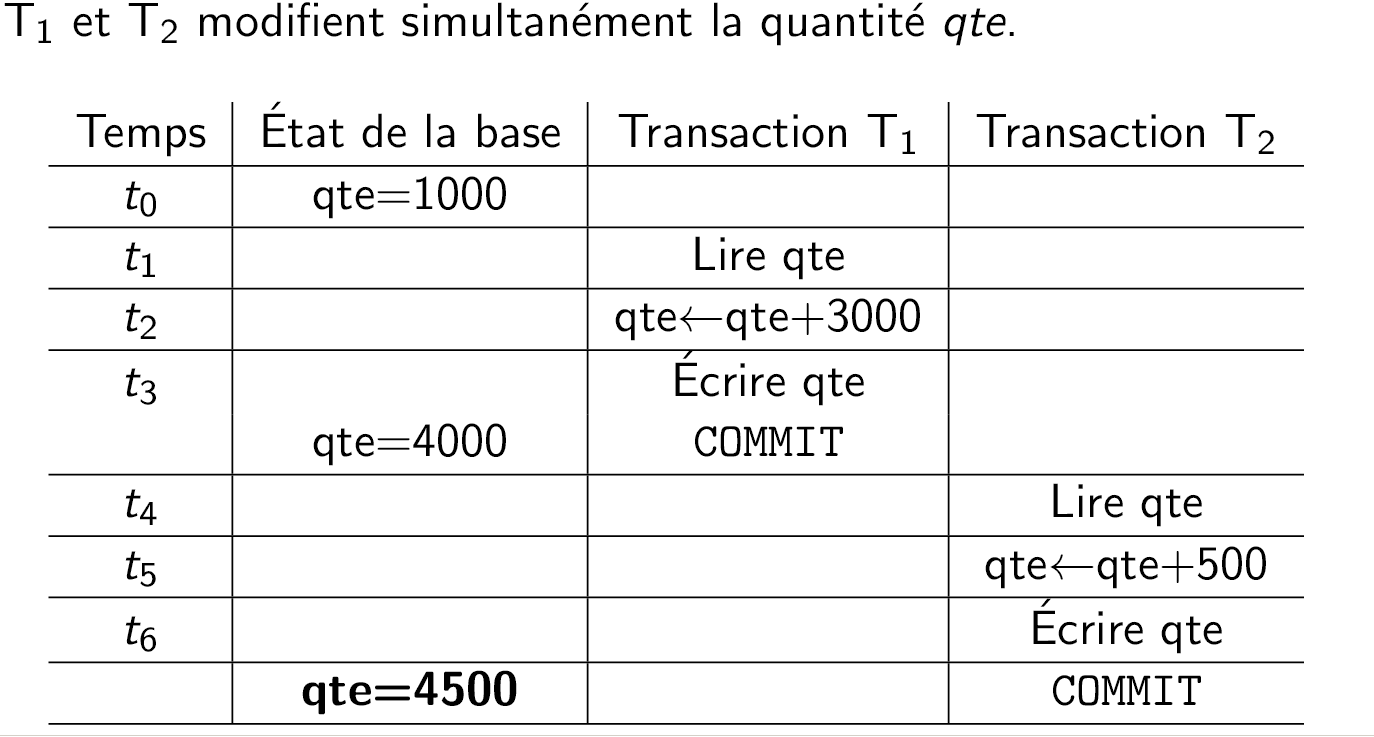
\includegraphics[scale=0.3]{./Pictures/BD1.PNG}\\
Donc dans cet exemple, 2 transactions veulent modifier simultanément la quantité qte. Le but étant d'avoir une quantité qte égale à 4500. Donc ici on a l'ordre des opérations à faire pour chacune des transactions. Cependant, il faut voir comment fonctionnent les verrous dans cet exemple.\\
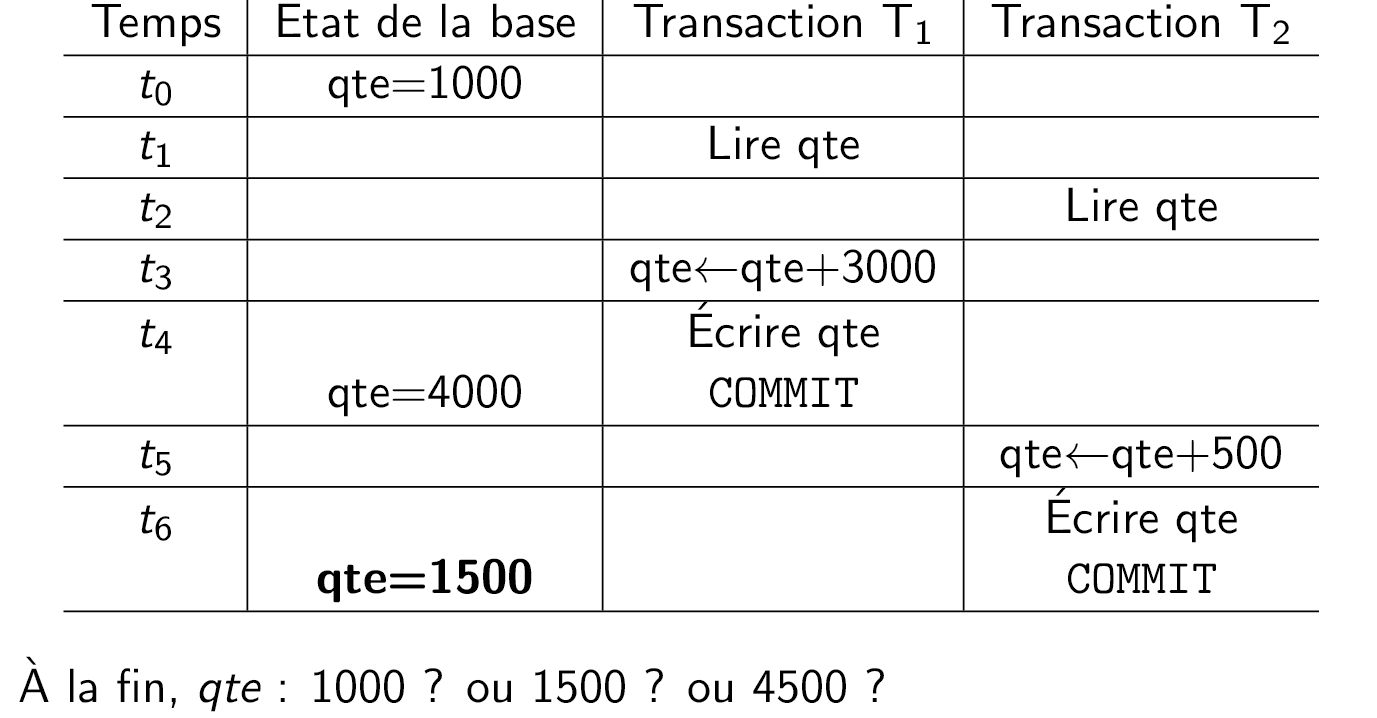
\includegraphics[scale=0.3]{./Pictures/BD2.PNG}\\
Dans ce tableau, à t0, qte = 1000. Ensuite à t1, la transaction T1 lit la valeur de qte (donc 1000), de même pour la transaction T2 à l'instant t2 (qte = 1000).\\
A l'instant t3, T1 modifie la valeur de qte (qte = qte + 3000) et à t4 enregistre cette modification par l'instruction COMMIT. Donc qte = 4000. A t5, T2 modifie aussi la valeur de qte et enregistre cette valeur.\\
Cependant on s'attendrait à avoir qte = 4500 mais non bande de gogols. Cette erreur intervient à l'instant t2. En effet, T2 lit la valeur actuel de qte, c'est-à-dire 1000. Donc sa modification de la valeur qte ne prend pas en compte la modification de T1. En effet, il y a une collision et donc une mauvaise gestion des verrous. La solution pour avoir qte = 4500 est la suivante.\\
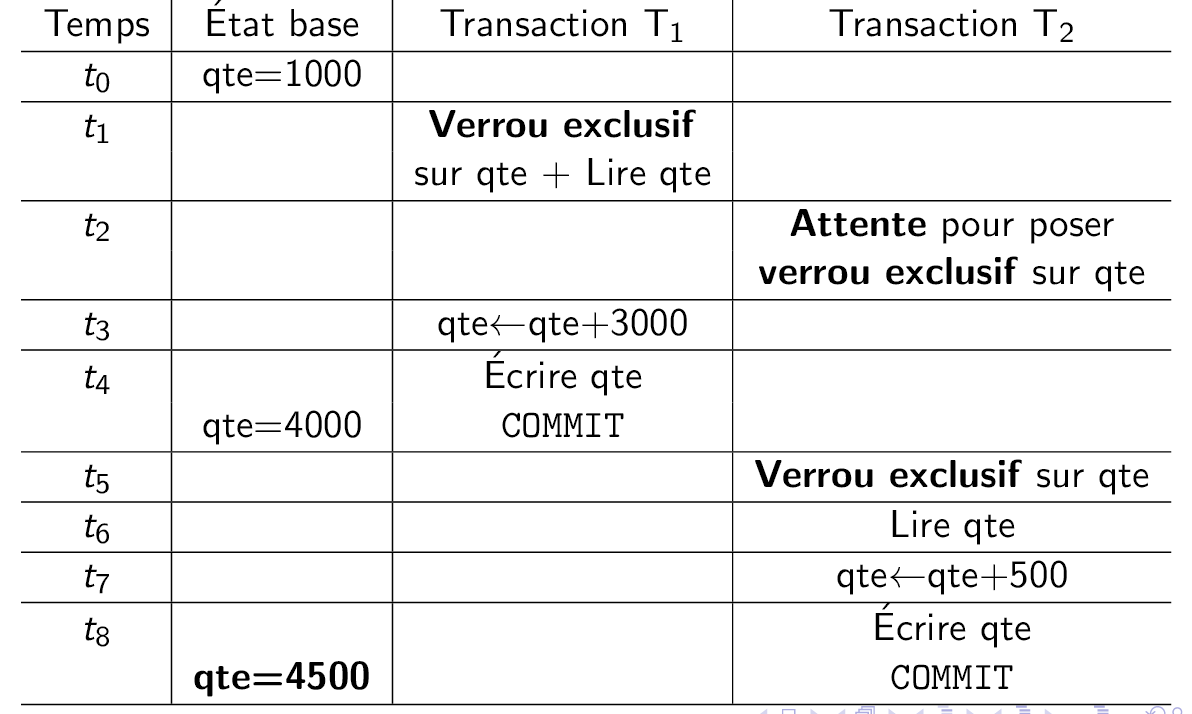
\includegraphics[scale=0.35]{./Pictures/BD3.PNG}\\ 
Dans cette version, T1 pose un verrou exclusif lors de la lecture de qte, c'est-à-dire, que T1 va appliquer une modification sur cette valeur et que T2 doit attendre la fin de ce verrou (COMMIT ou ROLLBACK). Après que T1 ait modifier la valeur et fait un COMMIT (qte = 4000), c'est au tour de T2 d'appliquer un verrou exclusif et de modifier la valeur de qte. Et comme par gicMa, qte = 4500, car la valeur à laquelle accède T2 a été modifié et validé par T1.\\\\
Pour les collisions de type : lecture impropre et lecture non reproductible se référait au cours parce que j'ai trop la flemme. Si vous avez compris cette exemple, vous comprendrez sûrement les autres (je vous conseille d'aller voir le cours pour tester vos connaissances ofc).\\\\
Vu que vous êtes chimiques, on va faire une suite d'exemples :
\begin{lstlisting}[style=MySQLStyle]
-- l'utilisateur 1 change le nom d'un film (numero 15 et realisateur 58)
-- on a ici l'application d'un verrou exclusif
UPDATE ens2004.film
SET titre = 'MABITE'
WHERE numFilm = 15
AND realisateur = 58;

-- l'utilisateur 1 et 2 executent la meme requete d'affichage
SELECT * FROM ens2004.film;
-- A ce moment la, la modification du film n'etant pas valide, le titre du film affiche est toujours l'ancien

-- l'utilisateur 1 fait un COMMIT
COMMIT;

SELECT * FROM ens2004.film;
-- La valeur etant modifie, l'affichage contiendra la nouvelle valeur c'est-a-dire MA...
\end{lstlisting}
Il existe plusieurs niveaux de cohérence pour une transaction.
Une donnée est dites salie si elle a été modifiée par une transaction non confirmée. En gros, par un COMMIT. Pour une transaction T, on peut exiger que T satisfasse une ou plusieurs des propriétés (c'est pas vraiment important mais c'est toujours utile):
\begin{enumerate}
\item : T ne modifie pas des données salies par d'autres transactions.
\item : T ne confirme pas ses changements avant la fin de la transaction.
\item : T ne lit pas des données salies pas d'autres transactions.
\item : D'autres transactions ne salissent pas des données lues par T avant que T soit terminée.\\
\end{enumerate}
Pour chacune de ces propriétés, un niveau de cohérence est attribué à T :
\begin{itemize}
\item niveau 0 si T vérifie 1 : donc pas de problèmes de perte de mise à jour.
\item niveau 1 si T vérifie 1 et 2 : si une transaction est annulée (ROLLBACK), il n'est pas nécessaire de défaire explicitement les modifications antérieures à l'annulation.
\item niveau 2 si T vérifie 1 et 2 et 3 : pas de problèmes de perte de mise à jour et de lecture impropre.
\item niveau 3 si T vérifie 1 et 2 et 3 et 4 : pas de problèmes de perte de mise à jour, de lecture impropre et assure la reproductibilité des lectures, donc une isolation totale de la transaction. (je vous avais dit de voir le cours)\\
\end{itemize}
Sur Oracle les verrous sont invoqués automatiquement dans des cas spécifiques, mais on peut le faire manuellement aussi. Ce tableau résume bien les différents verrous que l'on peut mettre.
\newline
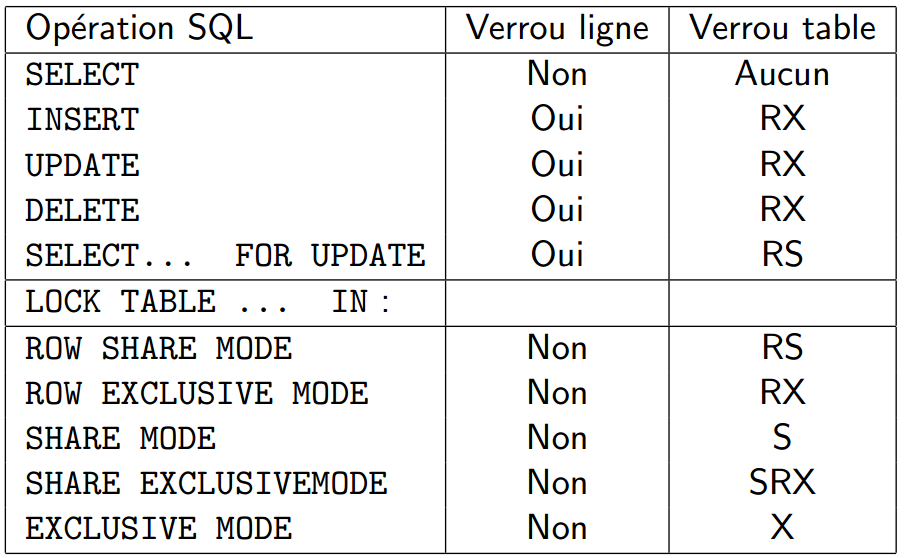
\includegraphics[scale=0.45]{./Pictures/BD4.png}
\newline
\begin{itemize}
\item RX : Row exclusif, interdiction de modification et de lecture sur la ligne que l'on modifie pour tout autre utilisateur
\item RS : Row share, interdiction de modification seulement sur la ligne que l'on lit
\item S : Share, interdiction de modification sur la table que l'on lit
\item X : Exclusif, interdiction de modification et lecture sur la table que l'on modifie
\end{itemize}

\subsubsection{Problème possible lié au verrou}
\textbf{Deadlock} : On rencontre ce problème lorsque un utilisateur attend la fin du verrou d'un autre alors que celui ci attend la fin du verrou de l'un. 
\newline Par Exemple je pose un verrou sur la ligne 1 d'une table puis un random pose un verrou sur la ligne 2. Je souhaite récupérer la valeur de la ligne 2 $\rightarrow$ je suis mis en attente par le random, sauf que ce putain de random attend que moi j'enlève mon verrou sur la ligne 1. Du coup on se retrouve en attente tout les deux comme des cons.
$\rightarrow$ Pour éviter ce problème il faut que l'ordre dans laquelle le random et moi posons les verrous soit le même. Je prend la ligne 1, il prend la ligne 1, je prend la ligne 2, il prend la ligne 2 etc... Cette solution est appelé \textbf{Règle de Havender}. Allez savoir pourquoi...
\newline
Prenons deux utilisateurs lambda :\\\\\\\
\begin{lstlisting}[style=MySQLStyle]
-- l'utilisateur 1 change le nom du film (numero 15 et realisateur 58)
UPDATE ens2004.film
SET titre = 'TD32'
WHERE numFilm = 15
AND realisateur = 58;

-- l'utilisateur 2 change le nom d'un autre film (numero 32 et realisateur 96)
UPDATE ens2004.film
SET titre = 'BOGOSS'
WHERE numFilm = 32
AND realisateur = 96;

-- l'utilisateur 1 change le nom du film qui est en train d'etre modifie par l'utilisateur 2 (numero 32 et realisateur 96)
UPDATE ens2004.film
SET titre = 'TD321'
WHERE numFilm = 32
AND realisateur = 96;

-- l'utilisateur 2 change le nom du film qui est en train d'etre modifie par l'utilisateur 1 (numero 15 et realisateur 58)
UPDATE ens2004.film
SET titre = 'BOGOSS1'
WHERE numFilm = 15
AND realisateur = 58;
\end{lstlisting}

Dans cet exemple, on ne fait pas de COMMIT. A partir de la troisième instruction, Oracle va tourner en boucle (il attend le COMMIT de l'utilisateur 2) et va afficher sur l'utilisateur 1 blocage fatale de même à la quatrième instruction.
Cette erreur est due au fait que deux utilisateurs veulent modifier des données qui sont modifiés par l'un et par l'autre mais n'ont fait aucune validation ou annulation.\\\\
\textbf{Problème de la tasse à café....} : Il s'agit du fait que la saisie d'un utilisateur peut potentiellement mettre indéfiniment le programme en pause (Par exemple, je vais prendre une tasse de thé parce que j'aime le thé et faire chier les gens), ce qui provoque dans le cas où on a posé un verrou avant la demande de saisie, cela verrouille la cible indéfiniment et donc bloqué d'autre utilisateur.
$\rightarrow$ Pour éviter ce problème, il faut poser le verrou après la saisie tout simplement. 

\chapter{Base de données Objet}

Objet ? Wut ? C'est quoi encore cette partie ? \\
Ne vous inquiétez pas ! La partie objet de la base de données n'est juste qu'une simple révision de vos cours d'informatique objet mais avec ce merveilleux langage SQL. \\
\section{Créer un type}
A quoi sa sert ? Bah sa sert à définir un type objet qui est abstrait. Il est défini pas l'utilisateur pour décrire la structure (ses attributs) et le comportement (ses méthodes).\\
Sa fameuse syntaxe :
\begin{lstlisting}[style=MySQLStyle]
CREATE [ OR REPLACE ] TYPE nomType AS OBJECT
(nomAttribut type [, nomAttribut type ....]);
\end{lstlisting}

Prenons un exemple : Nous voulons créer un type adresse avec une rue, une ville, un code postal et le nom de la ville :
\begin{lstlisting}[style=MySQLStyle]
CREATE TYPE obAdresseTy AS OBJECT(
Rue VARCHAR2(50),
Ville VARCHAR2(30),
CodePostal CHAR(5),
Pays VARCHAR2(15));
\end{lstlisting}
Comme vous le constatez, nous créons un type comme si c'était une table avec des attributs, la nature de l'attribut et la taille de l'attribut. AS OBJECT permet de définir le type comme un objet; c'est à dire comme un constructeur en Java qui va être utilisé dans d'autres types et tables quand c'est nécessaire. \\

Maintenant nous voulons créer un type personne qui possède un nom, un prénom et le type adresse qu'on a créé plus tôt.
\begin{lstlisting}[style=MySQLStyle]
CREATE TYPE obPersonneTy AS OBJECT(
Nom VARCHAR2(30),
Prenom VARCHAR2(30),
Adresse obAdresseTy);
\end{lstlisting}
Vous pouvez le remarquer aussi qu'un attribut est de nature un type. Cet attribut permet d'appeler le type qu'on souhaite pour éviter de réécrire tous les attributs d'adresse. En gros l'attribut adresse va appeler tous les attributs du type adresse. Plus simple non ? \\

Pour supprimer un type rien de spécial. Mais à faire si il n'est plus utilisé !
\begin{lstlisting}[style=MySQLStyle]
DROP TYPE nomObjetType;
\end{lstlisting}
Une erreur apparaitra si vous voulez supprimer un type qui est encore présent dans une table utilisée. Pour cela il faut supprimer la table puis le type.

\section{Créer une table avec des types}
Après avoir pris le temps de créer ces jolis types, nous voulons créer une table qui comporte la colonne personne à l'intérieur accompagné d'un login et de la date d'inscription.
\begin{lstlisting}[style=MySQLStyle]
CREATE TABLE obClient (
login CHAR(20) PRIMARY KEY ,
client obPersonneTy,
dateIns DATE NOT NULL);
\end{lstlisting}
Le code ci-dessus nous montre que la table peut appeler un type. A quoi sa sert ? Bah sa sert à raccourcir le code et d'éviter d'appeler tous les attributs qu'on a besoin. De manière plus abstraite, le table va appeler tous les attributs de type Personne qui va appeler tous les attributs de type Adresse. En gros nous avons économiser 7 lignes de création d'attributs qui va quand même apparaître dans la table. Elle n'est pas belle la vie ? \\
REMARQUE : Dans une table, il faut toujours avoir un attribut qui a le rôle de clé primaire (Genius gnégné) MAIS un type ne peut pas être une clé primaire (Je t'ai troué le cul là hein!).\\ \\
Maintenant qu'on a perdu du temps pour créer des tables, il faut savoir les remplir (de sp... spécialité maison). Regardez bien le code :
\begin{lstlisting}[style=MySQLStyle]
INSERT INTO obClient
VALUES ('toto',
obPersonneTy ('Duval', 'Thomas',
obAdresseTy('rue des dunes', 'Trouville', '76666', 'France')),
TO DATE('01/05/07','DD/MM/YY'));
\end{lstlisting}
Comme vous le constatez, pour donner des valeurs à une table c'est la même procédure SQL MAIS nous avons mis un type dans notre table et pour compléter les attributs de ce type, il faut juste l'appeler.\\
ATTENTION : Si un type possède un autre type dans ses attributs, il faut faire la même opération : appeler le type et compléter ses attributs. \\\\

Après avoir bien remplis (hohoho), faut savoir rechercher les données d'un type. C'est la même procédure mais faut faire un appel spécial pour le type.\\ \\

Pour chercher le nom d'un client :
\begin{lstlisting}[style=MySQLStyle]
SELECT p.client.Nom FROM obClient p;
\end{lstlisting}
Pour que le code marche à tous les coups, il faut donner une "abréviation" à notre table. Pourquoi ? Cela permet au code SQL de ne pas se confondre lors de l'exécution. Ici, nous avons mis comme abréviation la lettre p pour le client. Cela permettra de pouvoir cibler plus facilement ce qu'on cherche. Nous allons cibler dans ce cas l'attribut client qui est de type Personne dans la table et plus précisément nous voulons l'attribut nom du type Personne.\\ \\

Pour chercher la ville d'un client ;
\begin{lstlisting}[style=MySQLStyle]
SELECT p.client.Adresse.Ville FROM obClient p;
\end{lstlisting}
C'est la même procédure mais pour ce cas, nous voulions adresse. Pour le chercher, il faut passer par l'attribut client de type Personne qui contient Adresse qui celui la contient l'attribut ville. \\ \\

Maintenant pour modifier un type dans un table, c'est la même méthode mais faut spécifier l'appel tout simplement.\\
Modifions la rue d'un client tiens :
\begin{lstlisting}[style=MySQLStyle]
UPDATE obClient p
SET p.client.adresse.rue='15 rue des vagues'
WHERE UPPER (p.client.nom)='DUVAL';
\end{lstlisting}
Comme prévu, la méthode SQL pour modifier ne change pas mais faut juste faire la spécification comme dans la recherche.

\section{Créer une table avec un seul type d'objet}
La méthode ne change pas, juste spécifier le type d'objet à utiliser et donner une clé primaire.
\begin{lstlisting}[style=MySQLStyle]
CREATE TABLE nomTable OF nomTypeObjet;
\end{lstlisting}

ATTENTION : Si nous voulons créer une table avec un seul type d'objet MAIS le type concerné possède un attribut venant d'un autre type, là c'est la merde. Mais SQL a tout pensé, faut juste donner une référence à l'attribut qui possède le type. \\
Regardez le code ça sera plus simple à comprendre.
\begin{lstlisting}[style=MySQLStyle]
CREATE TYPE obIndividuTy AS OBJECT (
NumIndividu NUMBER(5),
Nom VARCHAR2(30),
Prenom VARCHAR2(30) );

CREATE TABLE obIndividu OF obIndividuTy
(NumIndividu PRIMARY KEY);

CREATE TYPE obFilmTy AS OBJECT (
NumFilm NUMBER(5),
Titre VARCHAR2(50),
realisateur REF obIndividuTy );

CREATE TABLE obFilm OF obFilmTy
(NumFilm PRIMARY KEY);
\end{lstlisting}
Comme vous le voyez, la table obFilm n'est que de type obFilmTy. Cela veut dire que cette table ne peut posséder que les attribut du type Film. Le problème c'est qu'il a le type Individu qui vient foutre la merde. Pourquoi il a un REF ?? Le REF a pour fonctionnalité de faire référence a un autre type qui possède aussi une table (ici c'est Individu). Donc avec le REF l'affaire est réglée.\\ \\

Maintenant pour donner des valeurs, c'est autre chose. Il faut d'abord donner les attributs du type. Ici il faut d'abord donner les attributs de Individu avant de donner les attributs Film.\\ \\
Le code pour individu :
\begin{lstlisting}[style=MySQLStyle]
INSERT INTO obIndividu VALUES
(1996,'LECONTE', 'PATRICE');
INSERT INTO obIndividu VALUES
(2871,'SPIELBERG','STEVEN');
INSERT INTO obIndividu VALUES
(2987,'PAGNOL', 'MARCEL');
\end{lstlisting}
Ici c'est simple on ajoute des données dans la table obIndividu.
Ensuite pour donner les attributs Film, c'est plus compliqué. Pour insérer les attributs, il faut donner la référence à l'individu qu'on souhaite. 
\begin{lstlisting}[style=MySQLStyle]
INSERT INTO obFilm
SELECT 43, 'LE MARI DE LA COIFFEUSE',
REF(b) FROM obIndividu b
WHERE NumIndividu=1996;
INSERT INTO obFilm
SELECT 84,'LA LISTE DE SCHINDLER',
REF(a) FROM obIndividu a
WHERE NumIndividu=2871;
INSERT INTO obFilm
SELECT 18,'CESAR',
REF(c) FROM obIndividu c
WHERE NumIndividu=2987;
\end{lstlisting}
Ce code nous explique que lorsqu'on ajoute un film, il faut faire référence (avec REF) sur l'individu qu'on souhaite car sinon, le film ne contient aucun réalisateur, c'est similaire à NullPointeurException de mes c...
\section{Création d'une spécification et d'un corps par des méthodes}
Une méthode permet de manipuler des types et de définir leur comportement à n'importe quel moment. Une méthode ne peut cependant effectuer des modifications sur la base de données.\\ \\

Pour créer un type avec sa spécification :
\begin{lstlisting}[style=MySQLStyle]
CREATE [OR REPLACE] TYPE nomType AS OBJECT
(nomAttribut type [, nomAttribut type ? ] ,
MEMBER specification de procedure | fonction
[MEMBER specification de procedure | fonction ? ]
[MAP MEMBER specification de fonction ]
[ , PRAGMA RESTRICT REFERENCES (
methode, mode [ , mode ? ] ] );
\end{lstlisting}
MAP : pour définir un critère de tri.
mode : pour augmenter/restreindre les possibilités des méthodes
(WNDS, WNPS, RNDS, RNPS).\\ \\

Exemple avec le type Personne et une fonction qui détermine si la Personne habite en Ile de France ou en Province :
\begin{lstlisting}[style=MySQLStyle]
CREATE [OR REPLACE] TYPE obPersonneTy AS OBJECT
Nom VARCHAR2(30),
Prenom VARCHAR2(30),
Adresse obAdresseTy)
MEMBER FUNCTION parisProvince RETURN VARCHAR2,
[ , PRAGMA RESTRICT REFERENCES(
parisProvince,WNDS,RNDS));
\end{lstlisting}
WNDS : pas de modification de la base de données
RNDS : ne doit pas consulter la base de données. \\ \\

Maintenant faut définir le corps :
\begin{lstlisting}[style=MySQLStyle]
CREATE [OR REPLACE] TYPE BODY nomType IS|AS
MEMBER corps de la procedure | fonction
[MEMBER corps de la procedure | fonction ? ]
[MAP MEMBER corps de la fonction de tri ]
\end{lstlisting}

Dans notre exemple nous voulons définir la fonction qui détermine où la Personne habite :
\begin{lstlisting}[style=MySQLStyle]
CREATE OR REPLACE TYPE BODY obPersonneTy IS
MEMBER FUNCTION parisProvince RETURN VARCHAR2 IS
		pp VARCHAR2(8)
	BEGIN
		if (SUBSTR(adresse.CodePostal,1,2) IN
				('77','78','75', '91','92', '93','94','95'))
			then pp:='idf';
			else pp:='province';
		end if;
	return pp
	END parisProvince;
END;
\end{lstlisting}

Nous pouvons faire pareil avec une fonction de tri.\\
Spécification :
\begin{lstlisting}[style=MySQLStyle]
CREATE OR REPLACE TYPE obAdresseTy AS OBJECT
Rue VARCHAR2(50),
Ville VARCHAR2(30),
Code Postal CHAR(5)
Pays VARCHAR2(15),
MAP MEMBER FUNCTION triAdresse RETURN VARCHAR2);
\end{lstlisting}

Corps :
\begin{lstlisting}[style=MySQLStyle]
CREATE OR REPLACE TYPE BODY obAdresseTy IS
	MAP MEMBER FUNCTION triAdresse RETURN VARCHAR2 IS
		BEGIN
		RETURN CodePostal||Ville;
	END triAdresse;
END;
\end{lstlisting}

Recherche :
\begin{lstlisting}[style=MySQLStyle]
SELECT p.client.Nom,
	p.client.parisProvince situation ,
	p.client.adresse.codePostal code FROM obClient p
ORDER BY p.client.adresse;
\end{lstlisting}



\end{document}
